\chapter{Evaluación}\label{sec:ev}

Se procedió a verificar el funcionamiento de un modelo de \omnetpp{} hecho en
Python. Para realizar esta tarea se implementó la simulación de ejemplo aloha
(parte de la distribución oficial de \omnetpp{}) en Python (la llamaremos
pyaloha).

Se puede mostrar teóricamente que para el protocolo de transmisión aloha el uso
óptimo del canal ($\frac{1}{e}$, aproximadamente $18.4\%$) ocurre cuando se
emite un paquete cada dos unidades de tiempo, mientras que para el protocolo
aloha ranurado, el uso óptimo ($\frac{1}{2e}$, aproximadamente $36,8\%$) ocurre
cuando se emite un paquete por unidad de tiempo [42]. Como se puede observar en
la figura~\ref{fig:channel_rate_aloha}, los datos simulados coinciden con los
cálculos teóricos.

\begin{figure}[h]
\centering
\caption{Simulación aloha (C++)}
\label{fig:channel_rate_aloha}
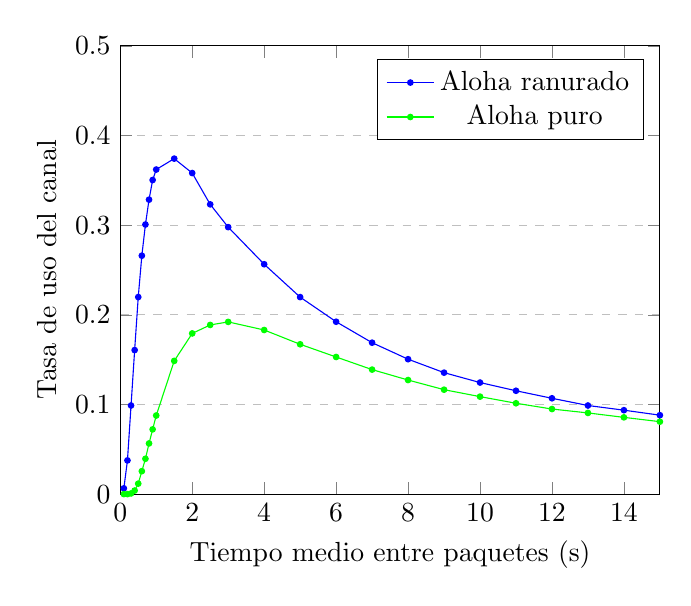
\begin{tikzpicture}
\begin{axis}[
    xlabel={Tiempo medio entre paquetes (s)},
    ylabel={Tasa de uso del canal},
    xmin=0, xmax=15,
    ymin=0, ymax=0.5,
    legend pos=north east,
    ymajorgrids=true,
    grid style=dashed,
]

\addplot[
    color=blue,
    mark=*,
    mark size=1pt
    ]
    coordinates {
        (0.1, 0.006466311480521) (0.2, 0.037610105670009) (0.3, 0.098827804181821) (0.4, 0.16064480261995) (0.5, 0.21978882360328) (0.6, 0.26590445965143) (0.7, 0.30069543988558) (0.8, 0.32841614300196) (0.9, 0.35030633100803) (1, 0.3620135096168) (1.5, 0.37417182276006) (2, 0.35808126966332) (2.5, 0.32315465311504) (3, 0.29777006758858) (4, 0.25638056059959) (5, 0.21972448797673) (6, 0.19226166810694) (7, 0.16888638161703) (8, 0.15047976608798) (9, 0.13547151185145) (10, 0.124433562124) (11, 0.11527294248685) (12, 0.10688476729002) (13, 0.098825058505501) (14, 0.093616973912472) (15, 0.088037337300734)
    };

\addplot[
    color=green,
    mark=*,
    mark size=1pt
    ]
    coordinates {
        (0.1, 0) (0.2, 0) (0.3, 0.00076325300354625) (0.4, 0.0039588643604514) (0.5, 0.011682838306187) (0.6, 0.025603452468452) (0.7, 0.039420787497505) (0.8, 0.056545297349915) (0.9, 0.072230508946743) (1, 0.087666903783682) (1.5, 0.14858681850652) (2, 0.17922565762884) (2.5, 0.18868286038616) (3, 0.19206834134435) (4, 0.18305322477005) (5, 0.16710512686259) (6, 0.15294315842394) (7, 0.13886721388324) (8, 0.12723940926008) (9, 0.11648069652152) (10, 0.1087283587839) (11, 0.10134104010002) (12, 0.094900113189545) (13, 0.090550009969597) (14, 0.085604136965468) (15, 0.080802896018396)
    };

\legend{Aloha ranurado, Aloha puro}
    
\end{axis}
\end{tikzpicture}
\end{figure}

\section{Verificación}

Para la implementación de pyaloha se siguió un patrón de traducción casi línea
por línea del código original en C++, para evitar introducir cambios
inadvertidos en el modelo.

Se ejecutó la simulación con los siguientes parámetros:

\begin{itemize}
    \item número de hosts: 15

    \item tasa de transmisión: 9600kbps

    \item tamaño de paquete: 952b

    \item tiempo total de simulación: 60min

    \item tiempo entre paquetes: variable exponencial con media $\lambda$,
donde $\lambda$ se hizo variar entre 0 y 15 (segundos)
\end{itemize}

Para cada valor de $\lambda$ se corrió la simulación 4 veces:

\begin{itemize}
    \item En C++, aloha puro
    \item En C++, aloha ranurado
    \item En Python, aloha puro
    \item En Python, aloha ranurado
\end{itemize}

\noindent y en cada experimento se recogió la tasa de utilización del canal
calculada por el programa.

El hallazgo fue que para el modelo pyaloha se obtuvieron los mismos resultados
que para el modelo aloha. No es que se obtuvieron resultados similares: se
obtuvieron exactamente los mismos resultados. Recordar que la inicialización
del generador de números aleatorios utiliza la misma semilla, por lo que los
eventos han sido generados en tiempos exactamente iguales, en ambos modelos.

Esto deja claro que la implementación del modelo en Python es tan funcional
como la implementación del modelo en C++.

\section{Rendimiento}

A continuación se presenta una comparación entre los modelos realizados con
\omnetpp{} (código en C++) y los mismos modelos escritos en Python, en términos de
velocidad de procesamiento. Las simulaciones se realizaron en una notebook con
procesador Intel i7-1065G7 CPU @ 1.30GHz, con 8GB de memoria RAM. Sin embargo,
los resultados se presentan en términos de eventos por segundo (una métrica que
\omnetpp{} escribe por salida estándar).

\subsection{Aloha}

Mientras menor es el tiempo medio entre paquetes, las simulaciones necesitan
más tiempo para finalizar. Esto es debido a que se generan más mensajes
(eventos) que deben ser procesados por el kernel de simulación hasta alcanzar
el tiempo límite de 60 minutos (simulados).

En la figura~\ref{fig:aloha_cpp_time} vemos que la ejecución más lenta del
modelo hecho en C++ corre en menos de un segundo:

\begin{figure}[h]
\centering
\caption{Tiempo de ejecución aloha (C++)}
\label{fig:aloha_cpp_time}
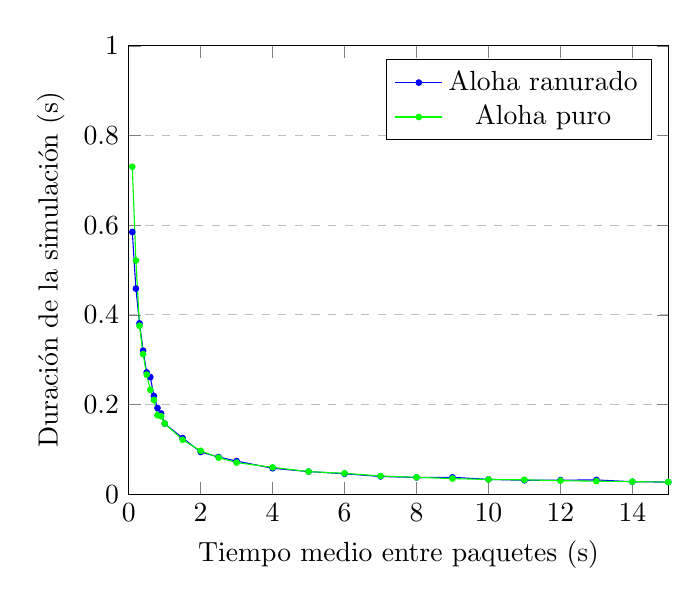
\begin{tikzpicture}
\begin{axis}[
    xlabel={Tiempo medio entre paquetes (s)},
    ylabel={Duración de la simulación (s)},
    xmin=0, xmax=15,
    ymin=0, ymax=1,
    legend pos=north east,
    ymajorgrids=true,
    grid style=dashed,
]

\addplot[
    color=blue,
    mark=*,
    mark size=1pt
    ]
    coordinates {
        (0.1, 0.5848276320002697) (0.2, 0.4584900680001738) (0.3, 0.3809897589999309) (0.4, 0.32006621599975915) (0.5, 0.2715306320005766) (0.6, 0.26100987900008477) (0.7, 0.21912263300055201) (0.8, 0.19208460500067304) (0.9, 0.1798737869994511) (1, 0.15734090299974923) (1.5, 0.12501570099993842) (2, 0.09409088400025212) (2.5, 0.08267888499995024) (3, 0.07369433799976832) (4, 0.05768032499963738) (5, 0.05032164899967029) (6, 0.045464001999789616) (7, 0.039412827999512956) (8, 0.03712264900059381) (9, 0.03749758800040581) (10, 0.03290581700002804) (11, 0.03088372000001982) (12, 0.031212740000228223) (13, 0.03161678299966297) (14, 0.027711645000636054) (15, 0.026821356999789714)
    };

\addplot[
    color=green,
    mark=*,
    mark size=1pt
    ]
    coordinates {
        (0.1, 0.7302508539996779) (0.2, 0.5210480169998846) (0.3, 0.3756052059998183) (0.4, 0.3123093889989832) (0.5, 0.2664828619999753) (0.6, 0.23273999100092624) (0.7, 0.21011473699945782) (0.8, 0.17592885900012334) (0.9, 0.17366348799987463) (1, 0.15758263200041256) (1.5, 0.12107748500056914) (2, 0.09663343200008967) (2.5, 0.08128265099912824) (3, 0.07034532000034233) (4, 0.05974540800161776) (5, 0.05028533099903143) (6, 0.04651024399936432) (7, 0.0404815130004863) (8, 0.03751071900114766) (9, 0.034700645999691915) (10, 0.032678042000043206) (11, 0.03193541699874913) (12, 0.029999125999893295) (13, 0.028916971999933594) (14, 0.02776208700015559) (15, 0.02700130499943043)
    };

\legend{Aloha ranurado, Aloha puro}
    
\end{axis}
\end{tikzpicture}
\end{figure}


En tanto que para pyaloha, el tiempo alcanzado ronda los 2 minutos, como se
aprecia en la figura~\ref{fig:aloha_py_time}.


\begin{figure}[h]
\centering
\caption{Tiempo de ejecución pyaloha (Python)}
\label{fig:aloha_py_time}
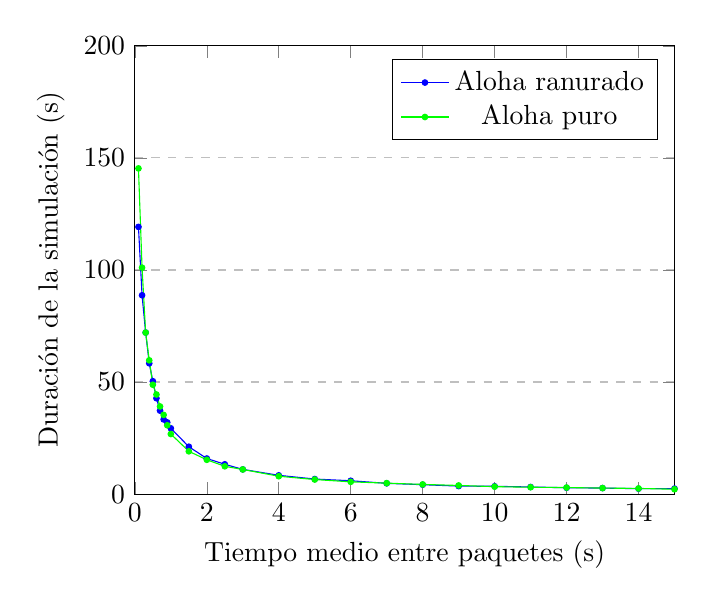
\begin{tikzpicture}
\begin{axis}[
    xlabel={Tiempo medio entre paquetes (s)},
    ylabel={Duración de la simulación (s)},
    xmin=0, xmax=15,
    ymin=0, ymax=200,
    legend pos=north east,
    ymajorgrids=true,
    grid style=dashed,
]

\addplot[
    color=blue,
    mark=*,
    mark size=1pt
    ]
    coordinates {
        (0.1, 119.21491560300001) (0.2, 88.72029479499997) (0.3, 72.0835129140005) (0.4, 58.36702549600068) (0.5, 50.37430065300032) (0.6, 42.77850106799997) (0.7, 37.25045305599997) (0.8, 33.3296159420006) (0.9, 32.00576179299969) (1, 29.37238604600043) (1.5, 21.154129888999705) (2, 15.896753297000032) (2.5, 13.319568406999679) (3, 11.031811740999728) (4, 8.387699105999673) (5, 6.728005928999664) (6, 5.965362578000168) (7, 4.820465584999511) (8, 4.209939122000833) (9, 3.5890565689996947) (10, 3.4924967070001003) (11, 3.1877669390005394) (12, 2.8483696450002753) (13, 2.701907260000553) (14, 2.4378241889999117) (15, 2.4747979300000225)
    };

\addplot[
    color=green,
    mark=*,
    mark size=1pt
    ]
    coordinates {
        (0.1, 145.31575596400035) (0.2, 101.02737987899945) (0.3, 72.07944632700037) (0.4, 59.69938408300004) (0.5, 48.79803602100037) (0.6, 44.44012174099953) (0.7, 39.112202779000654) (0.8, 35.348774288999266) (0.9, 30.71674825699847) (1, 26.81410339300055) (1.5, 19.10262854999928) (2, 15.320787870999993) (2.5, 12.419898019001266) (3, 11.003627136999057) (4, 7.984181870999237) (5, 6.520586059999914) (6, 5.483925722999629) (7, 4.905973154000094) (8, 4.3254758639996) (9, 3.870026284999767) (10, 3.3397165300011693) (11, 3.0784308909987885) (12, 2.9317122180000297) (13, 2.700906940001005) (14, 2.5422813530003623) (15, 2.188418952000575)
    };

\legend{Aloha ranurado, Aloha puro}
    
\end{axis}
\end{tikzpicture}
\end{figure}


Independientemente del tiempo medio entre mensajes, del tiempo total de la
simulación o de si el protocolo es ranurado o no, se puede observar que el
modelo implementado directamente en C++ procesa unos $1200000$ eventos por
segundo, mientras que el modelo implementado con Python es unas $200$ veces más
lento, procesando sólo $6000$ eventos por segundo.

\subsection{Tictoc}

Para Tictoc1, que consiste en un simple pasaje de mensajes entre dos instancias
de \verb!Txc!, encontramos que el modelo implementado en C++ procesa unos 5
millones de eventos por segundo, mientras que el que utiliza Python sólo
alcanza el medio millón, es decir, es unas $10$ veces más lento.

Tictoc2 introduce el uso herramientas para loggear información durante una
simulación. En particular, se presenta el constructo \verb!EV!.  En este caso,
la performance de C++ no se ve afectada, alcanzando también unos 5 millones de
eventos por segundo. En cambio, el modelo que utiliza Python sólo alcanza unos
$17.000$ mensajes por segundos (unas $300$ veces más lento). Esto se debe a que
en Python, \verb!EV! no está llamando directamente a código C++ de \omnetpp{}.
Como se dijo en la sección~\ref{subsec:ev}, en C++ es un macro y por lo tanto
es expandido en tiempo de compilación, mientra sque en Python es un objeto que
inspecciona el stack para conocer el contexto y recién entonces llama a una API
de C++.

En efecto, si el modelo en C++ dice:

\begin{minted}[linenos=false]{c++}
EV << getName() << "'s counter is " << counter << "\n";
\end{minted}

\noindent su traducción directa a Python resulta aproximadamente 1000 veces más
lenta

\begin{minted}[linenos=false]{Python}
EV << self.getName() << "'s counter is " << self.counter << '\n'
\end{minted}

\noindent mientras que la siguiente variante, aparentemente igual, es sólo 300
veces más lenta

\begin{minted}[linenos=false]{Python}
EV << f"{self.getName()}'s counter is {self.counter}\n"
\end{minted}

La diferencia viene dada por el hecho de que la primera variante (la que es más
lenta) consiste en 4 usos del operador \verb!<<! (left shift) sobre el objeto
\verb!EV!, cada uno de los cuales se traduce en una inspección del stack trace
para evaluar el contexto de ejecución, mientras que en la segunda variante se
utiliza \verb!<<! una única vez.

\subsection{Conclusión}

Como era de esperar, se encontró que los modelos implementados directamente en
C++ se terminan de simular más rápidamente. No obstante, qué tanto más rápido
no es un valor constante: la complejidad del método \verb!handleMessage! dicta
la magnitud de la penalidad en la performance. Esto es consistente con el hecho
de que mientras más tiempo pase la simulación ejecutando instrucciones Python
dentro del intérprete, más se aleja de la performance ideal alcanzada por un
modelo que utilice sólo C++ la totalidad del tiempo.

\section{Complejidad de código}

La siguiente comparación entre modelos de \omnetpp{} puro (C++) y \omnetpp{}
implementando modelos en Python se basa en la reimplementación de los
siguientes ejemplos de muestra incluidos en el código fuente de \omnetpp{}: aloha,
canvas, cqn, dyna, fifo, histograms, hypercube, routing, tictoc.

En ciertos fragmentos de código donde predomina la llamada a métodos y
funciones de \omnetpp{}, los modelos en C++ y los modelos en Python son
necesariamente casi idénticos, como se observa en el siguiente ejemplo:

\noindent C++:

\begin{minted}[linenos=false]{c++}
void NetBuilder::initialize()
{
    scheduleAt(0, new cMessage());
}
\end{minted}

\noindent Python:

\begin{minted}[linenos=false]{Python}
    def initialize(self):
        self.scheduleAt(0, cMessage())
\end{minted}

No obstante, notamos algunos factores que contribuyen a una mejora en la
complejidad de código: ausencia de caracteres como corchetes y punto y coma
para estructurar el código, ausencia de calificación del nombre de espacios
(\verb!Netbuilder::!).

En líneas generales, los modelos de ejemplo que incluye \omnetpp{} están diseñados
para mostrar cómo trabajar con \omnetpp{}, lo cual hace que el código consista
principalmente en llamadas a las APIs y, por lo tanto, su implementación usando
Python sea prácticamente igual en términos de cantidad de líneas.

Donde realmente vemos la diferencia es, por ejemplo, en el siguiente fragmento:

\begin{minted}[linenos=false]{c++}

    std::map<long, cModule *> nodeid2mod;
    std::string line;

    std::fstream nodesFile(par("nodesFile").stringValue(), std::ios::in);
    while (getline(nodesFile, line, '\n')) {
        if (line.empty() || line[0] == '#')
            continue;

        std::vector<std::string> tokens = cStringTokenizer(line.c_str()).asVector();
        if (tokens.size() != 3)
            throw cRuntimeError("wrong line in module file: 3 items required, line: \"%s\"", line.c_str());

        // get fields from tokens
        long nodeid = atol(tokens[0].c_str());
        const char *name = tokens[1].c_str();
        const char *modtypename = tokens[2].c_str();
        EV << "NODE id=" << nodeid << " name=" << name << " type=" << modtypename << "\n";

        // create module
        cModuleType *modtype = cModuleType::find(modtypename);
        if (!modtype)
            throw cRuntimeError("module type '%s' for node '%s' not found", modtypename, name);
        cModule *mod = modtype->create(name, parent);
        nodeid2mod[nodeid] = mod;

        // read params from the ini file, etc
        mod->finalizeParameters();
    }
\end{minted}

Python:

\begin{minted}[linenos=false]{Python}

    nodeid2mod = {}

    with open(self.par('nodesFile').stringValue(), 'r') as fh:
        for line in fh.readlines():
            line = line.strip()
            if not line or line.startswith('#'):
                continue

            nodeid, name, modtypename = line.split()
            nodeid = int(nodeid)

            EV << 'NODE id=' << nodeid << ' name=' << name << ' type=' << modtypename << '\n'

            # create module
            modtype = cModuleType.find(modtypename)
            if modtype is None:
                raise RuntimeError(f'module type '{modtypename}' for node '{name}' not found')

            mod = modtype.create(name, parent)
            nodeid2mod[nodeid] = mod

            # read params from the ini file, etc
            mod.finalizeParameters()

\end{minted}

donde Python es más simple por no declaración de variables, la facilidad de
lectura de archivos, la facilidad para manipulación de strings o, como vemos en
el siguiente ejemplo, por la facilidad para trabajar con diccionarios:

C++:

\begin{minted}[linenos=false]{c++}
    std::map<long, cModule *>::iterator it;

    for (it = nodeid2mod.begin(); it != nodeid2mod.end(); ++it) {
            cModule *mod = it->second;
            mod->buildInside();
    }
\end{minted}

Python:

\begin{minted}[linenos=false]{Python}
        for mod in nodeid2mod.values():
            mod.buildInside()
\end{minted}

Como puede apreciarse en la tabla~\ref{table:loc}, la cantidad de líneas
necesaria para implementar un modelo en Python siempre fue menor que para el
modelo original en C++.  En el análisis se tienen en cuenta únicamente archivos
\verb!.h!, \verb!.cc!, \verb!.msg! y \verb!.py!.

\begin{table}[h!]
\centering
\begin{tabular}{l|rrr}
Modelo & C++ & Python & Proporción\\
\hline

aloha     & 511  & 352  & 68,88\% \\
canvas    & 145  & 114  & 78,62\% \\
cqn       & 185  & 100  & 54,05\% \\
dyna      & 401  & 291  & 72,57\% \\
fifo      & 285  & 122  & 42,81\% \\
histogram & 158  & 139  & 87,97\% \\
hypercube & 368  & 263  & 71,47\% \\
routing   & 551  & 370  & 67,15\% \\
tictoc    & 1755 & 705  & 40,17\% \\
\end{tabular}
\caption{Cantidad de líneas de código en modelos reimplementados en Python}
\label{table:loc}
\end{table}

Además de las características ya mencionadas que hacen de Python un lenguaje
más simple de manejar, los modelos implementados en Python tienen menos
archivos y menos líneas.
